\documentclass[12pt,letterpaper]{article}

\usepackage[utf8]{inputenc}
\usepackage[T1]{fontenc}
\usepackage{amsmath}
\usepackage{amsfonts}
\usepackage{amssymb}
\usepackage{amsthm}
\usepackage[left=2cm,right=2cm,top=2cm,bottom=2cm,headheight=22pt]{geometry}
\usepackage{fancyhdr}
\usepackage{setspace}
\usepackage{lastpage}
\usepackage{graphicx}
\usepackage{caption}
\usepackage{subcaption}
\usepackage{paralist}
\usepackage{multicol}

\theoremstyle{definition}
\newtheorem{question}{Question}
\newtheorem{example}{Example}
\newtheorem{exercise}[question]{Exercise}
\newtheorem*{challenge}{Challenge}

\begin{document}

%Paramètres de mise en forme des paragraphes selon les normes françaises
\setlength{\parskip}{1ex plus 0.5ex minus 0.2ex}
\setlength{\parindent}{0pt}

%Paramètres relatifs aux en-têtes et pieds de page.
\pagestyle{fancy}
\lhead{Theron J Hitchman}
\chead{\Large Reading and Guided Practice \#3}
\rhead{Fall 2013}
\lfoot{\emph{Math and Decision Making}}
\cfoot{} 
\rfoot{\emph{\thepage\ of \pageref{LastPage}}}

\section*{Introduction}
We look at the structure of some basic solutions to the picture hanging puzzle with 2 nails.
We shall also discuss generalizing the puzzle and our techniques for understanding it.

\section*{Goals}
At the end of this assignment, a student should be able to:
\begin{compactitem}
\item demonstrate several genuinely different solutions to the picture hanging puzzle with two nails;
\item state clearly two different generalizations of the picture hanging puzzle to a situation where there are three nails; and
\item describe a system of diagrams and symbols for organizing potential solutions to the different picture hanging puzzles with three nails.
\end{compactitem}
It is possible that a student might also be able to:
\begin{compactitem}
\item solve one or both of the variants of a picture hanging puzzle with three nails;
\item state some variants of the picture hanging puzzle for four nails.
\end{compactitem}

\section*{Reading and Questions for 4 September}

\subsection*{Solutions for 2 Nails}

One solution to the picture hanging puzzle with two nails is represented by the symbol $ABA^*B^*$. Of course, given what we learned in the last reading, this is the same diagram as $BAB^*A^*$. (Just change the direction of travel along the wire.)
\begin{figure}[h]
\centering
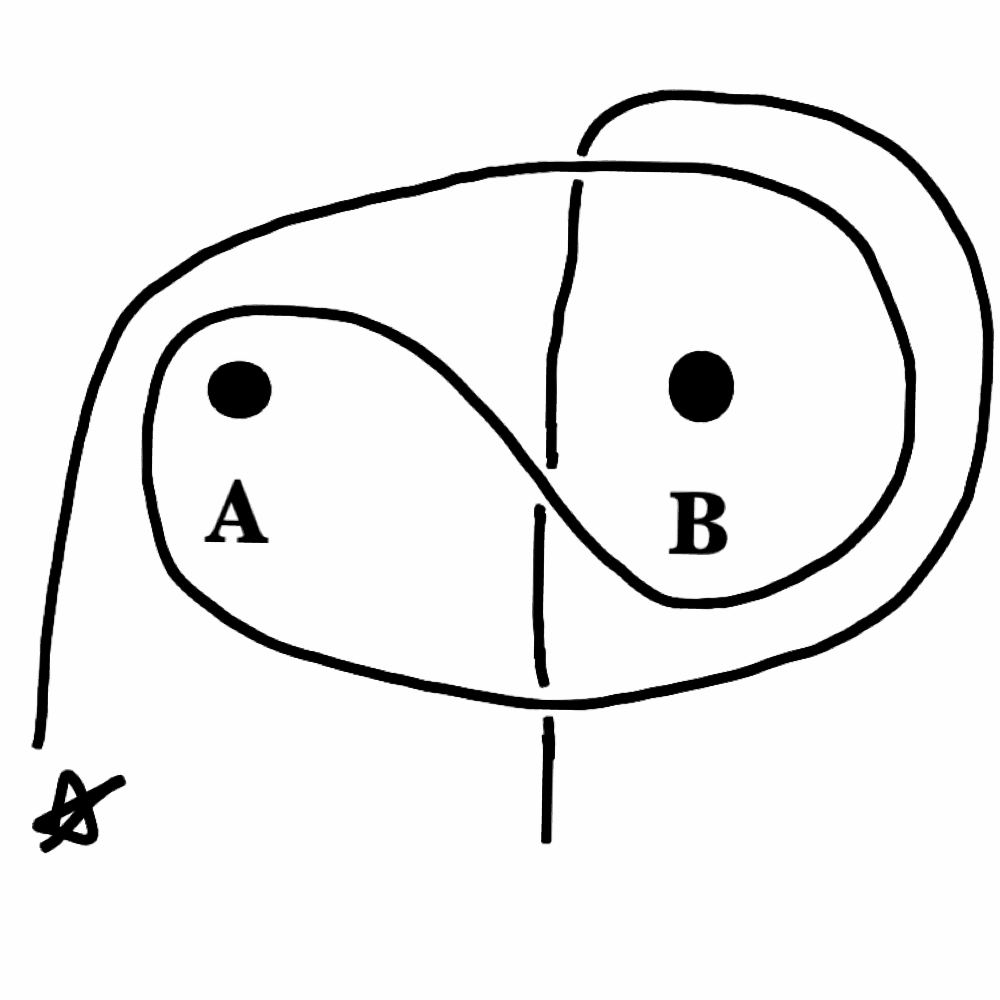
\includegraphics[height=2.5in]{rgp03pics/ABAsBs.png}
\caption{A Solution!}
\end{figure}
The key to this solution is twofold:
\begin{compactitem}
\item Alternating between the nails $A$ and $B$ to make sure the picture will hang,
\item Alternating between the unstarred ("moving right") and starred ("moving left") types of the letter.
\end{compactitem}
How do we see this in the symbols? 
If we remove the nail A, then we get $ABA^*B^* \longrightarrow BB^*$, which is sure to fall down. 
The wire just makes a loop over nail B but not around it.  
All of the coils around A become slack and can be pulled out.

Similarly, if we remove the nail B, then we get $ABA^*B^* \longrightarrow AA^*$, which is a loop over nail A but not around it. 
All of the coils around B become slack and can be pulled out.

\begin{exercise}
Using this understanding, find solutions of the picture hanging puzzle for 2 nails which have \textbf{exactly four letters} and whose beginnings are listed below:
\begin{compactitem}
\begin{multicols}{3}
\item $AB^*$
\item $A^*B$
\item $A^*B^*$
\item $BA^*$
\item $B^*A$
\item $B^*A^*$
\end{multicols}
\end{compactitem}
\end{exercise}

\begin{question}
Now we have eight different symbols that should represent solutions to the 2 nail picture hanging puzzle. 
We noted above that $ABA^*B^*$ and $BAB^*A^*$ are really the same physical solution. 
Do any of the six new solutions you just made pair up in a similar way?
\end{question}

\begin{challenge}
Find a solution to the 2 nail picture hanging puzzle whose symbols starts out with $AAAAB$.
\end{challenge}

\subsection*{Generalizing}

As satisfying as it is to solve a puzzle, mathematicians are never just ``done.''
Any good puzzle should have a family of related puzzles, and if we think carefully, we might find some of these interesting and approachable, too.

The most obvious thing we can change in the picture hanging puzzle is the number of nails.
Recall the original statement.
\begin{quotation}
\noindent
\textbf{2 Nail Picture Hanging Puzzle (PHP2):} Is there a way to arrange the wire around the two nails so that (1) with both nails the picture hangs from the wall, but (2) if \textbf{either} nail is removed the picture will fall down?
\end{quotation} 

If we simply replace ``two'' by ``three,'' we get this puzzle.
\begin{quotation}
\noindent
\textbf{3 Nail Picture Hanging Puzzle (PHP3):} Is there a way to arrange the wire around the three nails so that (1) with all nails the picture hangs from the wall, but (2) if \textbf{any single} nail is removed the picture will fall down?
\end{quotation} 

There is another, slightly subtler, generalization.
In PHP2, we only remove one nail, because 1 is just slightly greater than 0.
(Removing 0 nails is boring.)
But of course, $1=2-1$, also.
So in generalizing to three nails, this is another place we can replace a 2 by a 3.
If we change this equation to read $2 = 3 -1$, we get the suggestion that we should be removing two nails at a time.
We get this puzzle.
\begin{quotation}
\noindent
\textbf{3-remove-2 Picture Hanging Puzzle (PHP3-2):} Is there a way to arrange the wire around the two nails so that (1) with both nails the picture hangs from the wall, and (2) if any single nail is removed the picture will still hang, but (3) if \textbf{any pair} of nails is removed the picture will fall down?
\end{quotation} 

\begin{question}
What do you think we should mean by the puzzles PHP4, PHP4-2, and PHP4-3?
\end{question}


\subsection*{Diagrams \& Symbols for Three Nails}

The idea here is to work just as before, but use the symbols $A$, $B$ \emph{and $C$} for the three nails.

Rules:
\begin{compactitem}
\item pick a loose end of the wire to start at (this determines your direction of travel)
\item as you trace along, record the names of nails as you go \underline{over} them,
\item leave the letter plain if you are moving left-to-right, add a ${}^*$ if you are moving right-to-left.
\end{compactitem}

\begin{example}
This potential solution diagram has symbol $ACB^*A^*C$.
\begin{figure}[h]
\centering
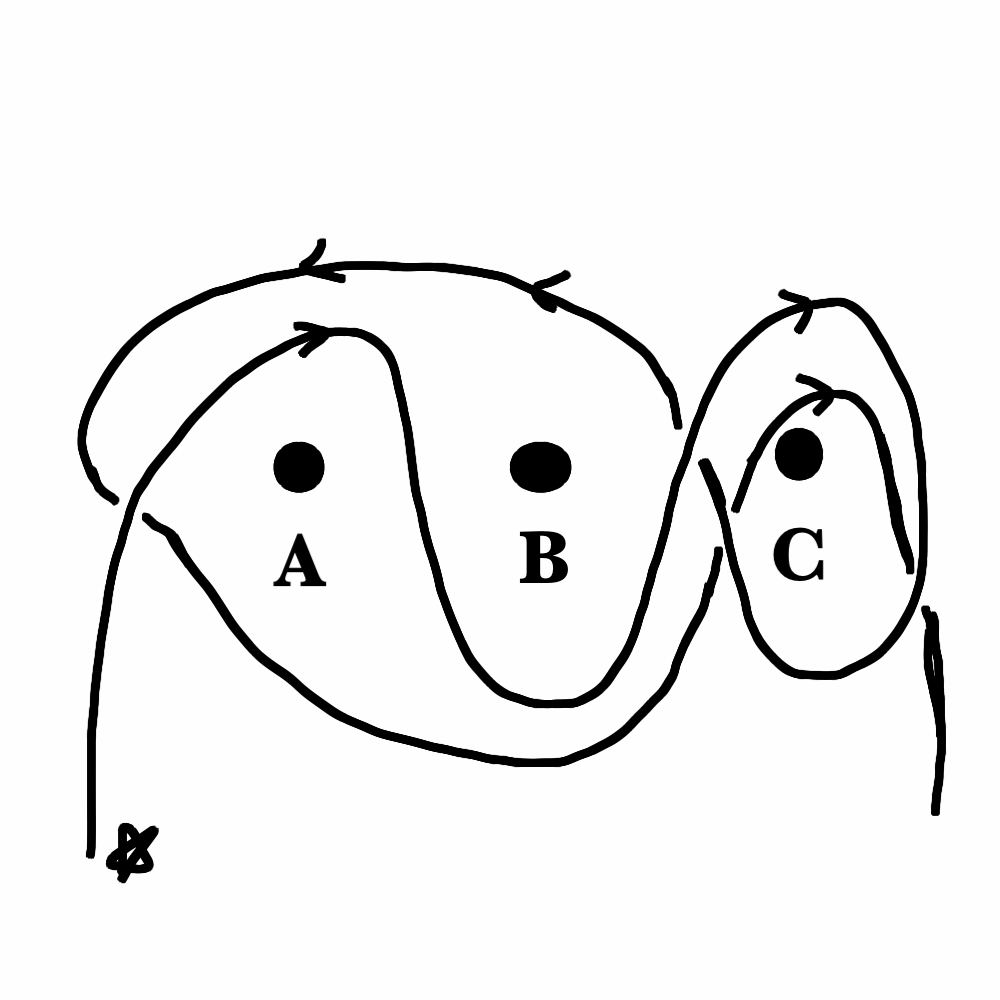
\includegraphics[height=2in]{rgp03pics/ACBsAsC.png}
\caption{An Example with 3 Nails}
\end{figure}
\end{example}

\begin{exercise}\label{exercise:mainex}
Verify that the symbol for the diagram below is $BC^*B^*A$.
\begin{figure}[h]
\centering
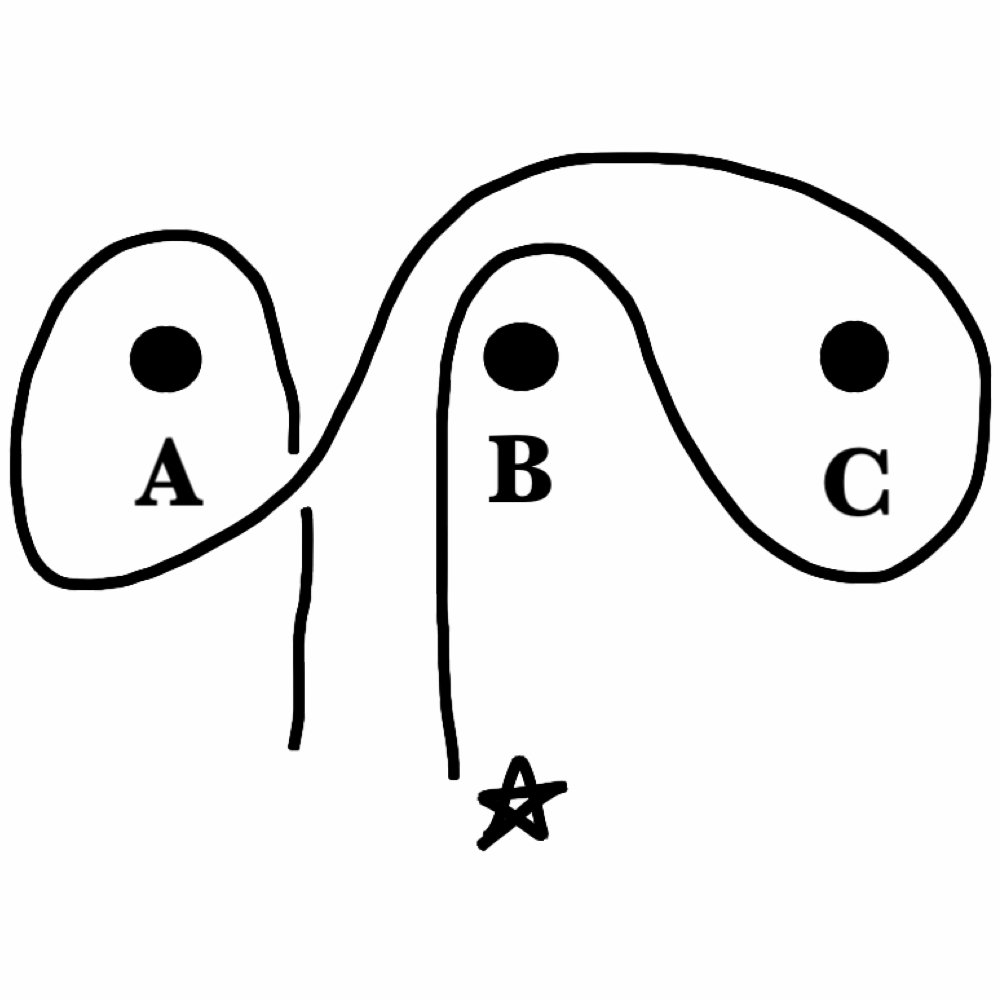
\includegraphics[height=2in]{rgp03pics/BCsBsA.png}
\caption{An Example with 3 Nails}
\end{figure}
\end{exercise}

\begin{exercise}
What is the symbol you get if you read the diagram from Exercise \ref{exercise:mainex} by traveling in the other direction?
\end{exercise}

\begin{exercise}
Suppose that you pull nail C from the diagram in Exercise \ref{exercise:mainex}. Verify that the result is a diagram for PHP2 whose symbol is just $A^*$.
\end{exercise}

\begin{exercise}
Draw diagrams for the symbols $CAB^*$ and $BCA^*$.
\end{exercise}

\begin{challenge}
Solve the puzzle PHP3.
\end{challenge}

%\begin{thebibliography}{9}
%\end{thebibliography}

\end{document}


















